\section{Motion Under a Central Force}

\noindent
We'll now study the motion of an object moving under the influence of a {\color{blue}\it central
force\/}; that is, a force whose magnitude at any point $P$ other than the origin depends only on
the distance from $P$ to the origin, and whose direction at $P$ is parallel to the line connecting
$P$ and the origin, as indicated in Figure~\ref{figure:6.4.1} for the case where the direction of
the force at every point is toward the origin. Gravitational forces are central forces; for example,
as mentioned in Section~4.3, if we assume that Earth is a perfect sphere with constant mass density
then Newton's law of gravitation asserts that the force exerted on an object by Earth's
gravitational field is proportional to the mass of the object and inversely proportional to the
square of its distance from the center of Earth, which we take to be the origin.

If the initial position and velocity vectors of an object moving under a central force are parallel,
then the subsequent motion is along the line from the origin to the initial position. Here we'll
assume that the initial position and velocity vectors are not parallel; in this case the subsequent
motion is in the plane determined by them. For convenience we take this to be the $xy$-plane. We'll
consider the problem of determining the curve traversed by the object. We call this curve the
{\color{blue}\it orbit\/}.

\begin{figure}[tbp]
  \centering
  \color{blue}
  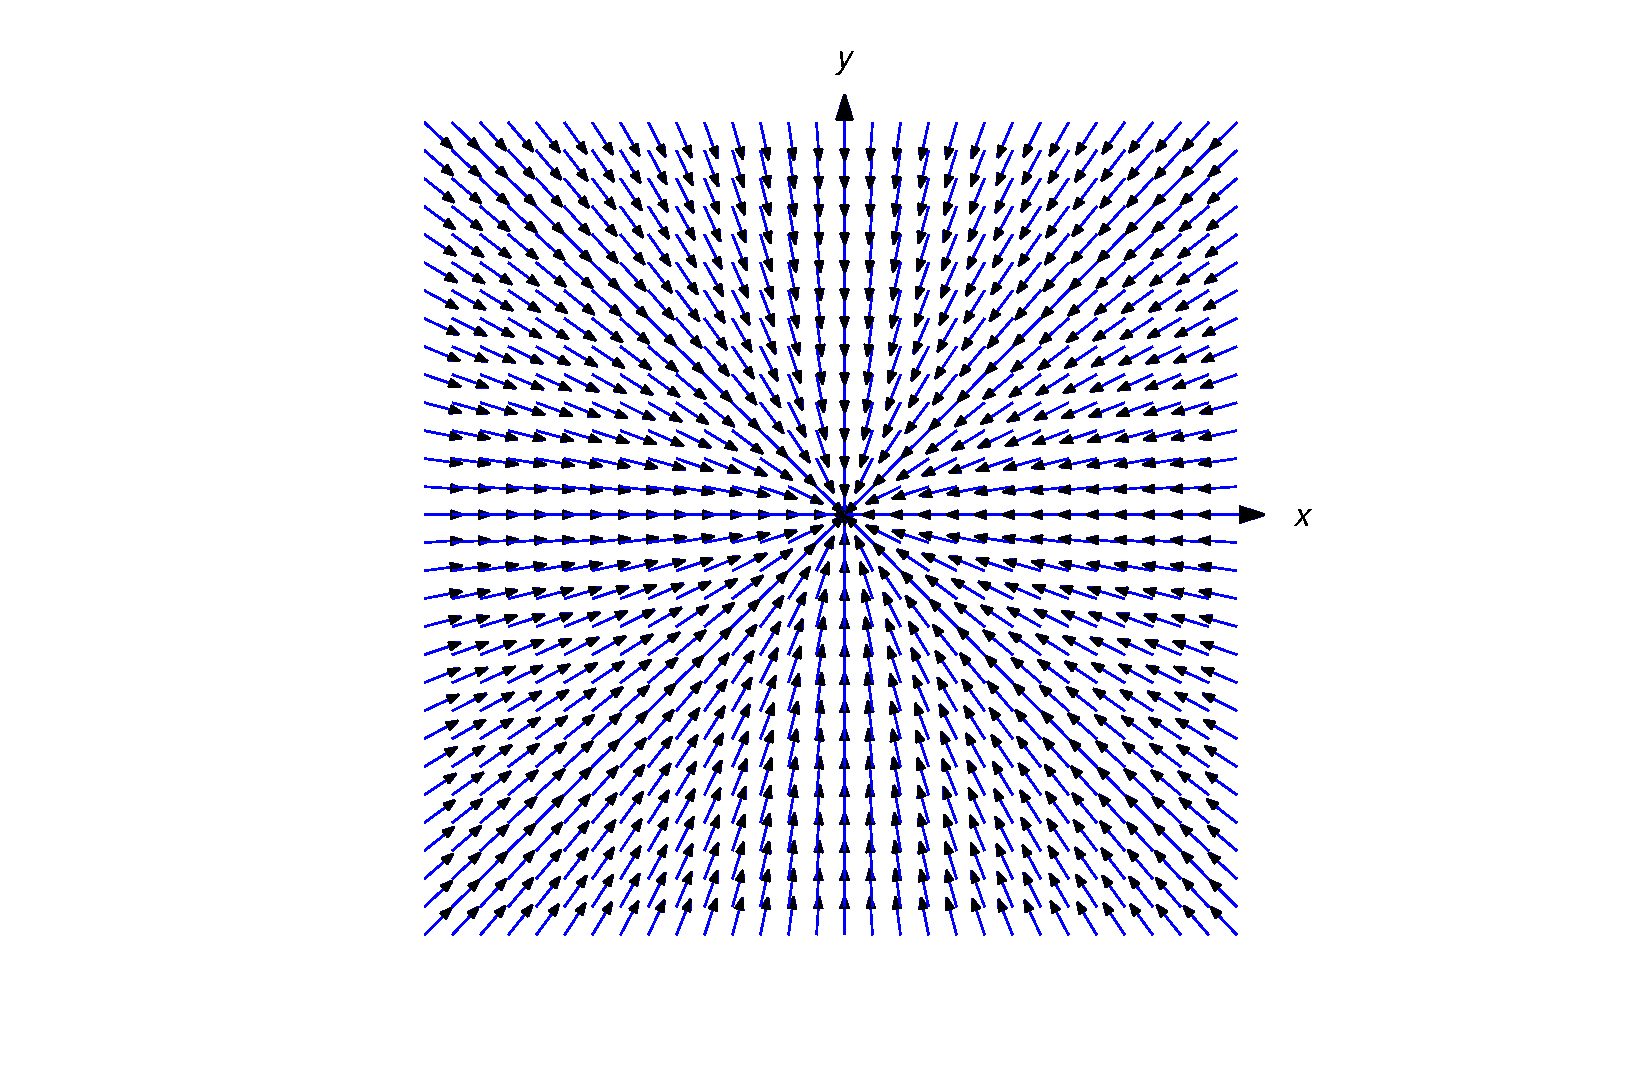
\includegraphics[bb=-78 148 689 643, width=5.67in, height=3.66in, keepaspectratio]{fig060401}
  \caption{}
  \label{figure:6.4.1}
\end{figure}

We can represent a central force in terms of polar coordinates
\[
  x=r\cos\theta,\quad y=r\sin\theta
\]
as
\[
  {\bf F}(r,\theta)=f(r)(\cos\theta\,{\bf i}+\sin\theta\,{\bf j}).
\]
We assume that $f$ is continuous for all $r>0$. The magnitude of ${\bf F}$ at
$(x,y)=(r\cos\theta,r\sin\theta)$ is $|f(r)|$, so it depends only on the distance $r$ from the point
to the origin; the direction of ${\bf F}$ is from the point to the origin if $f(r)<0$, or from the
origin to the point if $f(r)>0$. We'll show that the orbit of an object with mass $m$ moving under
this force is given by
\[
  r(\theta)=\frac{1}{u(\theta)},
\]
where $u$ is a solution of the differential equation
\begin{equation}
  \label{eq:6.4.1}\frac{d^{2}u}{d\theta^{2}}+u=-\frac{1}{mh^{2}u^{2}}f(1/u),
\end{equation}
and $h$ is a constant defined below.

Newton's second law of motion (${\bf F}=m{\bf a}$) says that the polar coordinates $r=r(t)$ and
$\theta=\theta(t)$ of the particle satisfy the vector differential equation
\begin{equation}
  \label{eq:6.4.2}m(r\cos\theta\,{\bf i}+r\sin\theta\,{\bf j})''= f(r)(\cos\theta\,{\bf i}+\sin\theta\,{\bf j}).
\end{equation}
To deal with this equation we introduce the unit vectors
\[
  {\bf e}_{1}=\cos\theta\,{\bf i}+\sin\theta\,{\bf j}\mbox{\quad and \quad}{\bf e}_{2}=-\sin\theta\,{\bf i}+\cos\theta\,{\bf j}.
\]
Note that ${\bf e}_{1}$ points in the direction of increasing $r$ and ${\bf e}_{2}$ points in the
direction of increasing $\theta$ (Figure~\ref{figure:6.4.2}); moreover,
\begin{equation}
  \label{eq:6.4.3}\frac{d{\bf e}_{1}}{d\theta}={\bf e}_{2},\quad \frac{d{\bf e}_{2}}{d\theta}=-{\bf e}_{1},
\end{equation}
and
\[
  {\bf e}_{1}\cdot{\bf e}_{2}=\cos\theta(-\sin\theta)+\sin\theta\cos\theta=0,
\]
so ${\bf e}_{1}$ and ${\bf e}_{2}$ are perpendicular. Recalling that the single prime $(')$ stands
for differentiation with respect to $t$, we see from \eqref{eq:6.4.3} and the chain rule that
\begin{equation}
  \label{eq:6.4.4}{\bf e}_{1}'=\theta'{\bf e}_{2}\mbox{\quad and \quad}{\bf e}_{2}'=-\theta'{\bf e}_{1}.
\end{equation}

\begin{figure}[tbp]
  \centering
  \color{blue}
  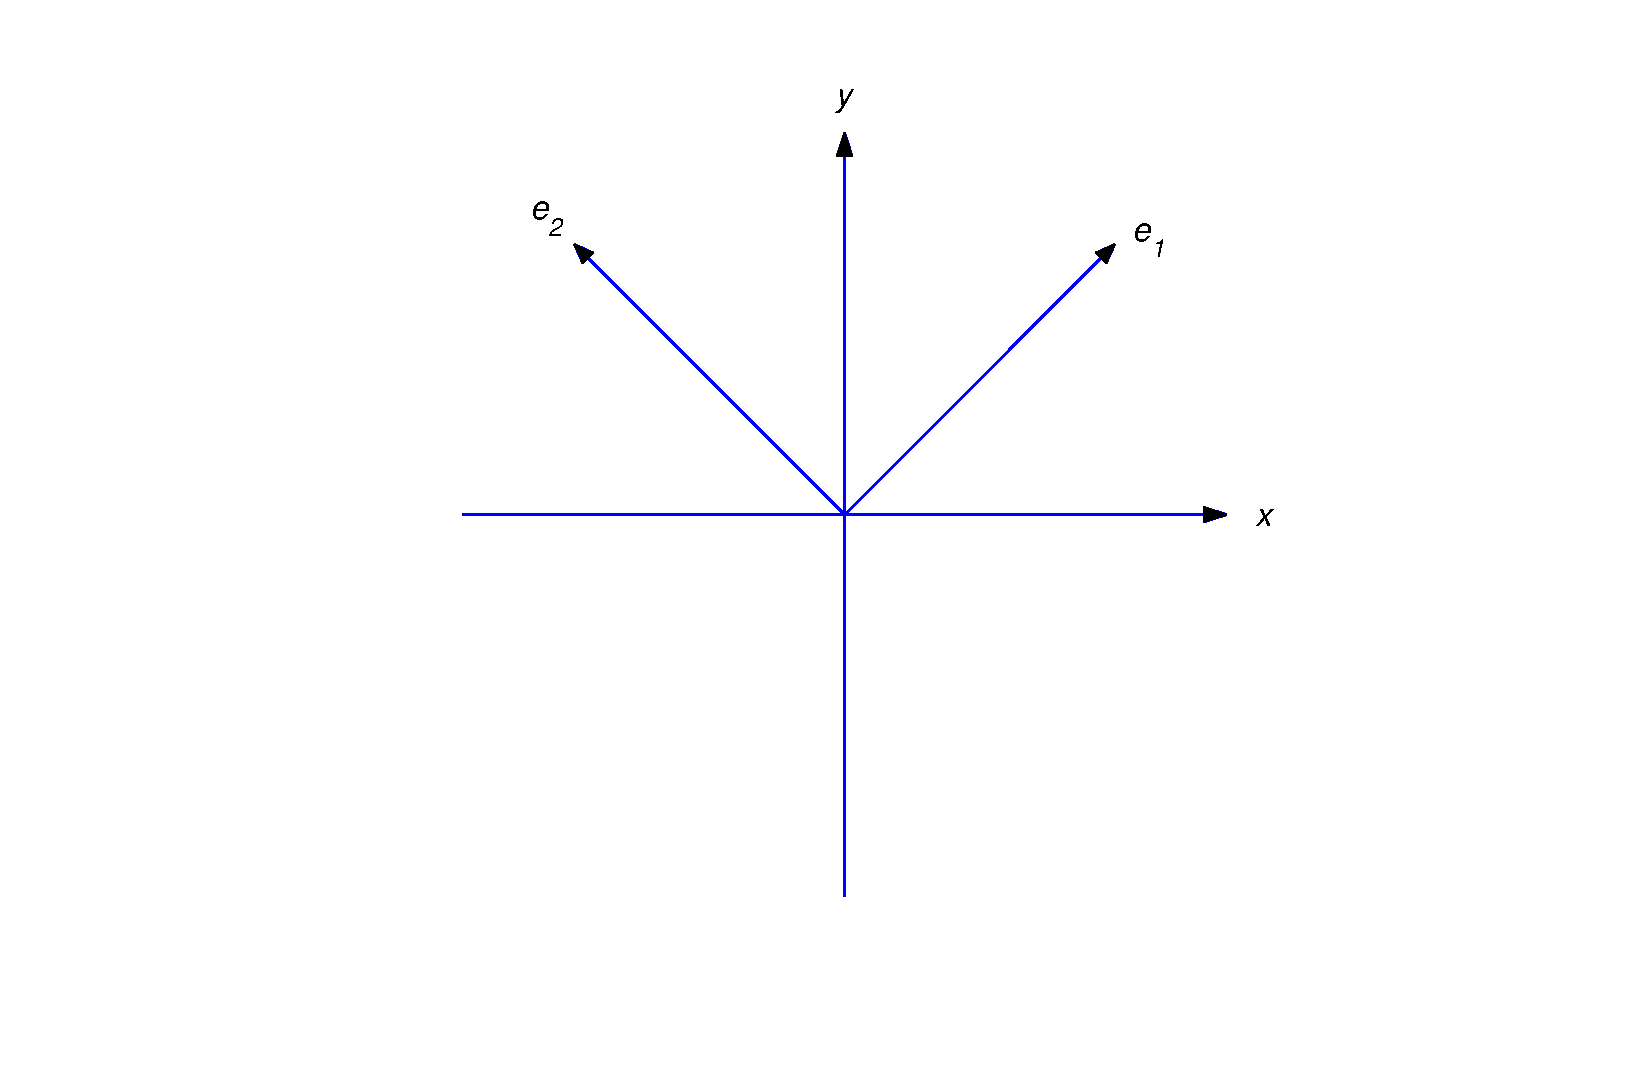
\includegraphics[bb=-78 148 689 643, width=5.67in, height=3.66in, keepaspectratio]{fig060402}
  \caption{}
  \label{figure:6.4.2}
\end{figure}

Now we can write \eqref{eq:6.4.2} as
\begin{equation}
  \label{eq:6.4.5}m(r{\bf e}_{1})''=f(r){\bf e}_{1}.
\end{equation}
But
\[
  (r{\bf e}_{1})'=r'{\bf e}_{1}+r{\bf e}_{1}'=r'{\bf e}_{1}+r\theta'{\bf e}_{2}
\]
(from \eqref{eq:6.4.4}), and
\begin{eqnarray*}
  (r{\bf e}_{1})'' & = & (r'{\bf e}_{1}+r\theta'{\bf e}_{2})'                                                                                               \\
                   & = & r''{\bf e}_{1}+r'{\bf e}_{1}'+(r\theta''+r'\theta'){\bf e}_{2}+r\theta'{\bf e}_{2}'                                                \\
                   & = & r''{\bf e}_{1}+r'\theta'{\bf e}_{2}+(r\theta''+r'\theta'){\bf e}_{2}-r(\theta')^{2}{\bf e}_{1}\mbox{\quad (from \eqref{eq:6.4.4})} \\
                   & = & \left(r''-r(\theta')^{2}\right){\bf e}_{1}+(r\theta''+2r'\theta'){\bf e}_{2}.
\end{eqnarray*}
Substituting this into \eqref{eq:6.4.5} yields
\[
  m\left(r''-r(\theta')^{2}\right){\bf e}_{1}+m(r\theta''+2r'\theta'){\bf e}_{2}=f(r){\bf e}_{1}.
\]
By equating the coefficients of ${\bf e}_{1}$ and ${\bf e}_{2}$ on the two sides of this equation we
see that
\begin{equation}
  \label{eq:6.4.6}m\left(r''-r(\theta')^{2}\right)=f(r)
\end{equation}
and
\[
  r\theta''+2r'\theta'=0.
\]
Multiplying the last equation by $r$ yields
\[
  r^{2}\theta''+2rr'\theta'=(r^{2}\theta')'=0,
\]
so
\begin{equation}
  \label{eq:6.4.7}r^{2}\theta'=h,
\end{equation}
where $h$ is a constant that we can write in terms of the initial conditions as
\[
  h=r^{2}(0)\theta'(0).
\]
Since the initial position and velocity vectors are
\[
  r(0){\bf e}_{1}(0)\mbox{\quad and \quad}r'(0){\bf e}_{1}(0)+r(0)\theta'(0){\bf e}_{2}(0),
\]
our assumption that these two vectors are not parallel implies that $\theta'(0)\ne0$, so $h\ne0$.

Now let $u=1/r$. Then $u^{2}=\theta'/h$ (from \eqref{eq:6.4.7}) and
\[
  r'=-\dst\frac{u'}{u^{2}}=-h\left(\frac{u'}{\theta'}\right),
\]
which implies that
\begin{equation}
  \label{eq:6.4.8}r'=-h\frac{du}{d\theta},
\end{equation}
since
\[
  \frac{u'}{\theta'}=\frac{du}{dt}\left/\frac{d\theta}{dt}\right.= \frac{du}{d\theta}.
\]
Differentiating \eqref{eq:6.4.8} with respect to $t$ yields
\[
  r''=-h\frac{d}{dt}\left(\frac{du}{d\theta}\right) =-h\frac{d^{2}u}{d\theta^{2}}\theta',
\]
which implies that
\[
  r''=-h^{2}u^{2}\frac{d^{2}u}{d\theta^{2}}\mbox{\quad since\quad}\theta'=hu^{2}.
\]
Substituting from these equalities into \eqref{eq:6.4.6} and recalling that $r=1/u$ yields
\[
  -m\left(h^{2}u^{2}\frac{d^{2}u}{d\theta^{2}}+\frac{1}{u}h^{2}u^{4}\right) =f(1/u),
\]
and dividing through by $-mh^{2}u^{2}$ yields \eqref{eq:6.4.1}.

Eqn.~\eqref{eq:6.4.7} has the following geometrical interpretation, which is known as
\href{https://mathshistory.st-andrews.ac.uk/Biographies/Kepler/}{\color{blue}
\it Kepler's Second Law\/}.

\begin{theorem}
  \color{blue}
  \label{thmtype:6.4.1} The position vector of an object moving under a central force sweeps out
  equal areas in equal times. More precisely, if $t_{1}<t_{2}$, the signed area swept from
  $\theta(t_{1})$ to $\theta(t_{2})$ {\rm (Figure~\ref{figure:6.4.3})} is given by
  \[
    A=\frac{h(t_{2}-t_{1})}{2},
  \]
  where $h=r^{2}\theta'$, which we have shown to be constant.
\end{theorem}

\begin{figure}[tbp]
  \centering
  \color{blue}
  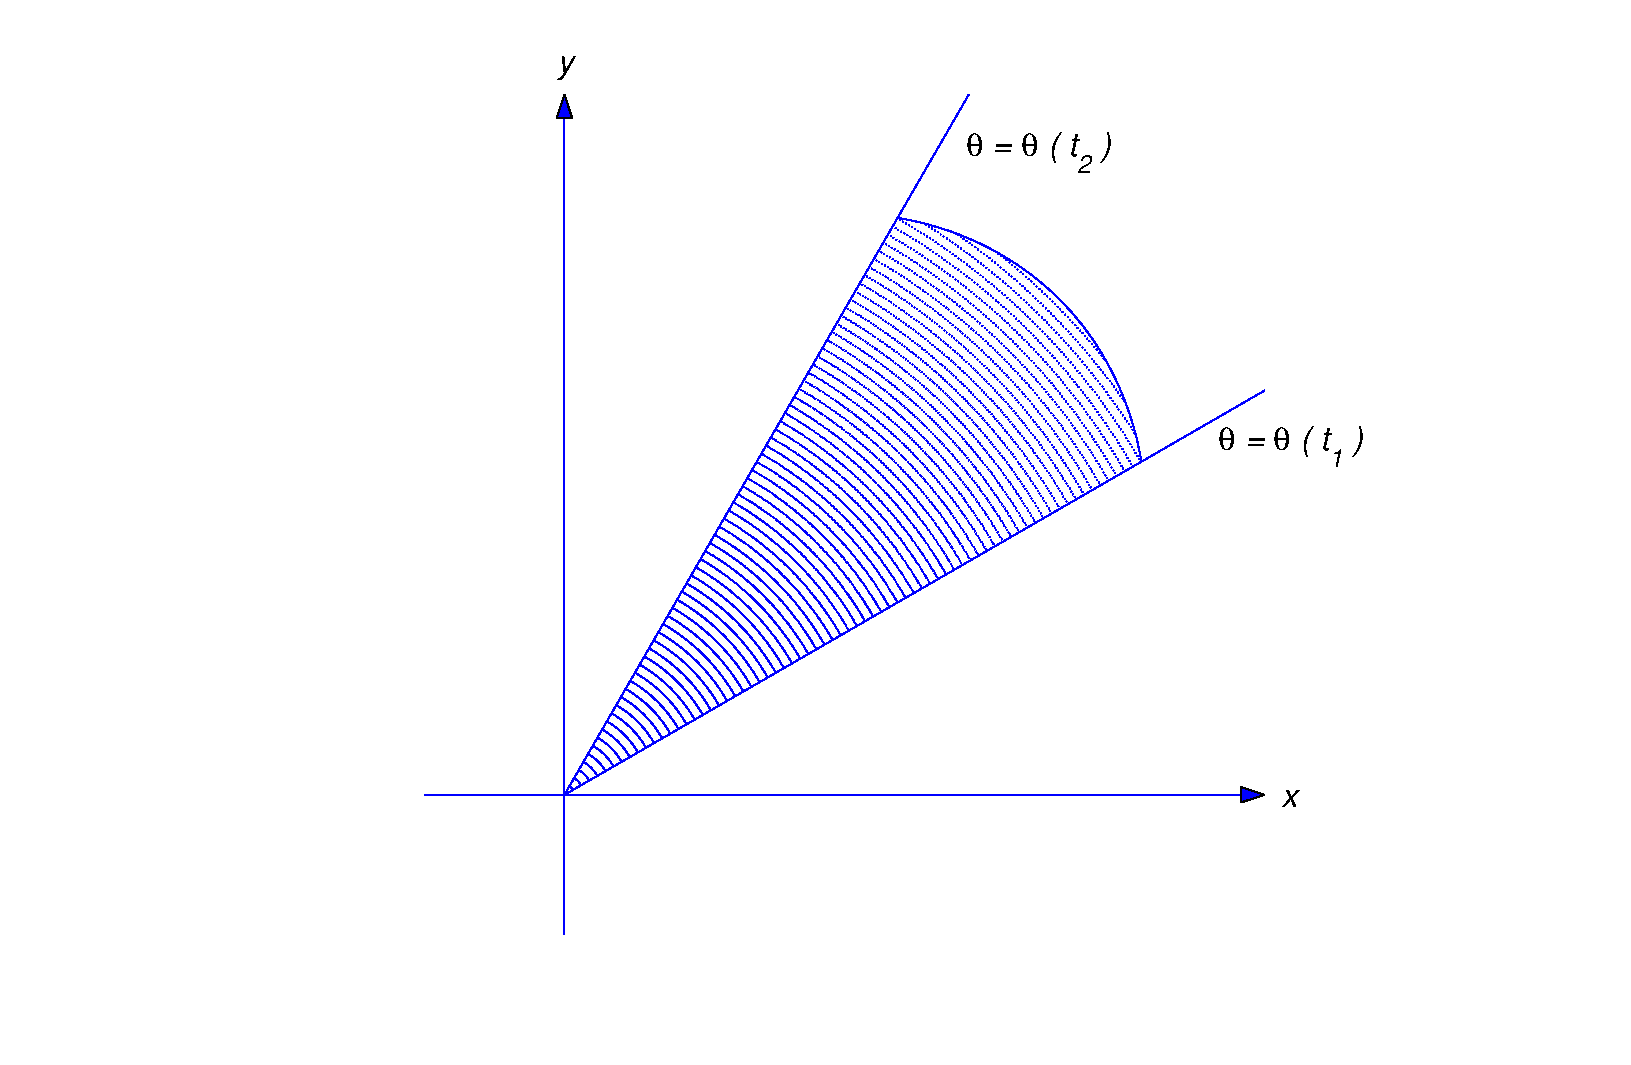
\includegraphics[bb=-78 148 689 643, width=5.67in, height=3.66in, keepaspectratio]{fig060403}
  \caption{}
  \label{figure:6.4.3}
\end{figure}

\proof Recall from calculus that the area of the shaded sector in Figure~\ref{figure:6.4.3} is
\[
  A=\frac{1}{2}\int_{\theta(t_{1})}^{\theta(t_{2})}r^{2}(\theta)\,d\theta,
\]
where $r=r(\theta)$ is the polar representation of the orbit. Making the change of variable
$\theta=\theta(t)$ yields
\begin{equation}
  \label{eq:6.4.9}A=\frac{1}{2}\int_{t_{1}}^{t_{2}}r^{2}(\theta(t))\theta'(t)\,dt.
\end{equation}
But \eqref{eq:6.4.7} and \eqref{eq:6.4.9} imply that
\[
  A=\frac{1}{2}\int_{t_{1}}^{t_{2}}h\,dt=\frac{h(t_{2}-t_{1})}{2},
\]
which completes the proof.

\boxit{Motion Under an Inverse Square Law Force}

\noindent
In the special case where $f(r)=-mk/r^{2}=-mku^{2}$, so ${\bf F}$ can be interpreted as a
gravitational force, \eqref{eq:6.4.1} becomes
\begin{equation}
  \label{eq:6.4.10}\frac{d^{2}u}{d\theta^{2}}+u=\frac{k}{h^{2}}.
\end{equation}
The general solution of the complementary equation
\[
  \frac{d^{2}u}{d\theta^{2}}+u=0
\]
can be written in amplitude--phase form as
\[
  u=A\cos(\theta-\phi),
\]
where $A\ge0$ and $\phi$ is a phase angle. Since $u_{p}=k/h^{2}$ is a particular solution of
\eqref{eq:6.4.10}, the general solution of \eqref{eq:6.4.10} is
\[
  u=A\cos(\theta-\phi)+\frac{k}{h^{2}};
\]
hence, the orbit is given by
\[
  r=\left(A\cos(\theta-\phi)+\frac{k}{h^{2}}\right)^{-1},
\]
which we rewrite as
\begin{equation}
  \label{eq:6.4.11}r=\frac{\rho}{1+e\cos(\theta-\phi)},
\end{equation}
where
\[
  \rho=\frac{h^{2}}{k}\mbox{\quad and \quad}e=A\rho.
\]
A curve satisfying \eqref{eq:6.4.11} is a conic section with a focus at the origin
(Exercise~\ref{exer:6.4.1}). The nonnegative constant $e$ is the {\color{blue}\it eccentricity\/} of
the orbit, which is an ellipse if $e<1$ (a circle if $e=0$), a parabola if $e=1$, or a
hyperbola if $e>1$.

\begin{figure}[H]
  \centering
  \color{blue}
  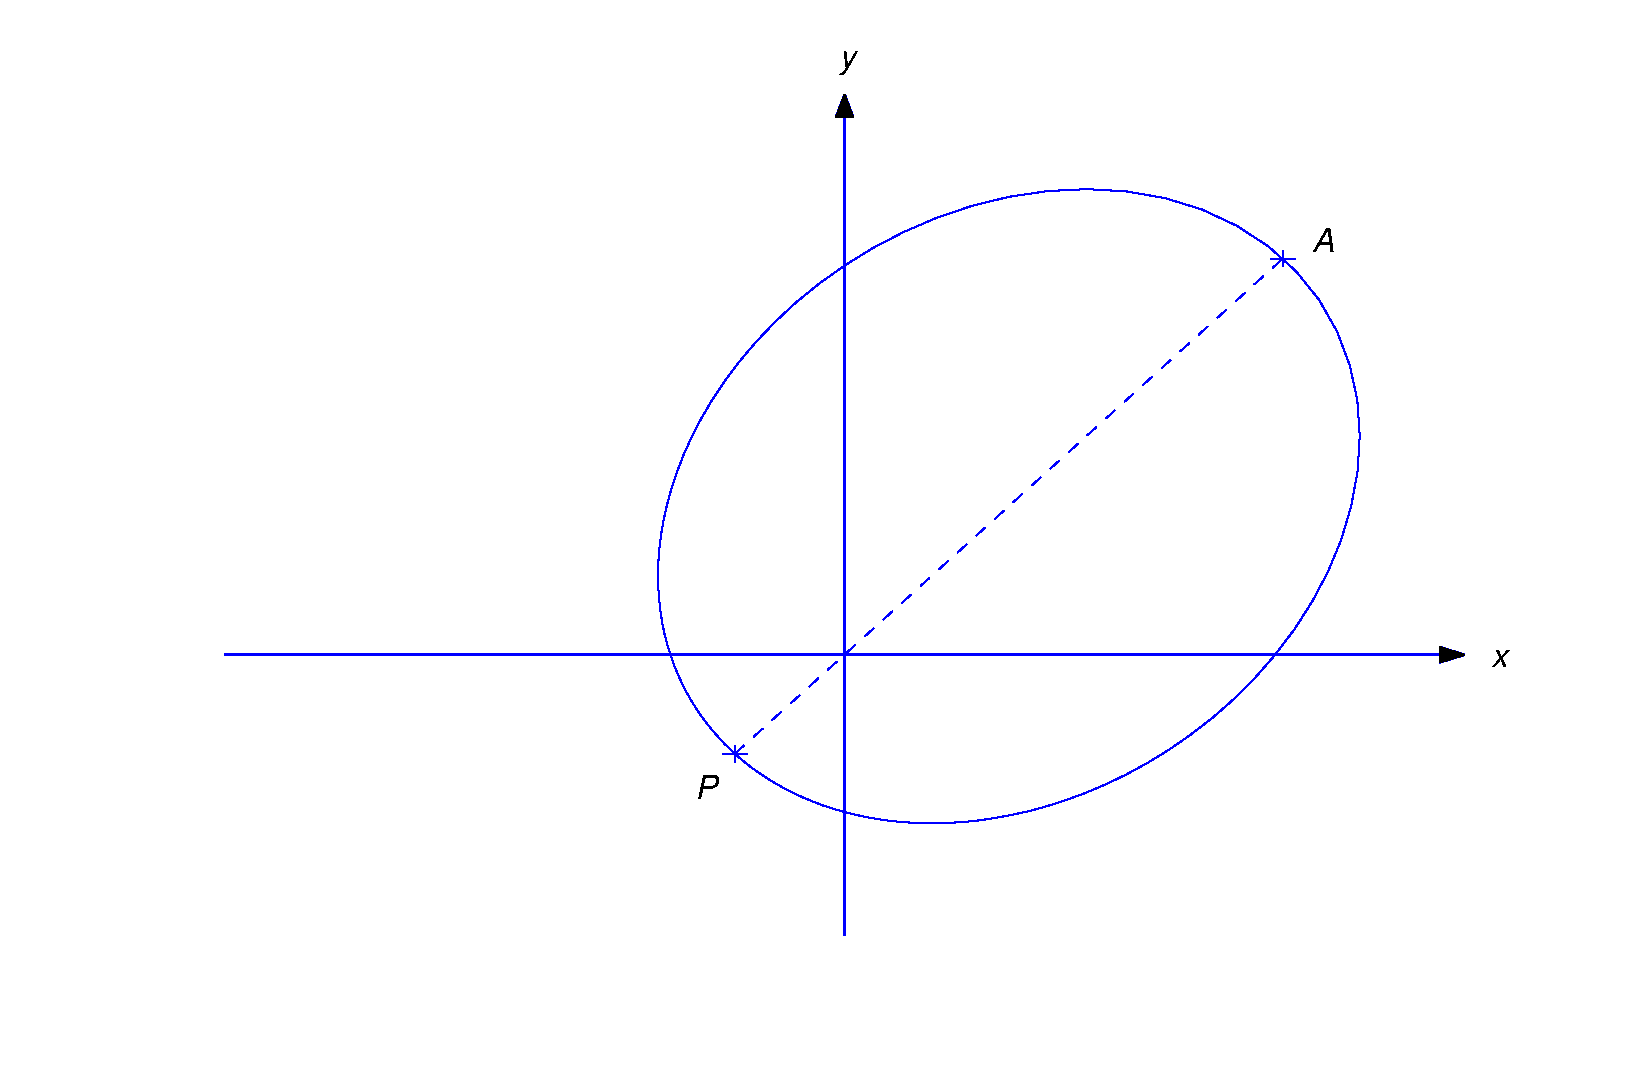
\includegraphics[bb=-78 148 689 643, width=5.67in, height=3.66in, keepaspectratio]{fig060404}
  \caption{}
  \label{figure:6.4.4}
\end{figure}

If the orbit is an ellipse, then the minimum and maximum values of $r$ are
\begin{eqnarray*}
  r_{\min} & = & \frac{\rho}{1+e}\quad\mbox{(the {\color{blue}\it periapsis distance\/}, attained when $\theta=\phi$)} \\
  r_{\max} & = & \frac{\rho}{1-e}\quad\mbox{(the {\color{blue}\it apoapsis distance\/}, attained when $\theta=\phi+\pi$)}.
\end{eqnarray*}
Figure~\ref{figure:6.4.4} shows a typical elliptic orbit. The point $P$ on the orbit where
$r=r_{\min}$ is the {\color{blue}\it periapsis\/} and the point $A$ where $r=r_{\max}$ is the
{\color{blue}\it apoapsis\/}.

For example, Earth's orbit around the Sun is approximately an ellipse with $e\approx.017$,
$r_{\min}\approx91\times10^{6}$ miles, and $r_{\max}\approx95\times10^{6}$ miles. Halley's comet has
a very elongated approximately elliptical orbit around the sun, with $e\approx.967$,
$r_{\min}\approx55\times10^{6}$ miles, and $r_{\max}\approx33\times10^{8}$ miles. Some comets (the
nonrecurring type) have parabolic or hyperbolic orbits.

\exercises
\begin{exerciselist}
  \item\label{exer:6.4.1} Find the equation of the curve
  \[
    r=\frac{\rho}{1+e\cos(\theta-\phi)}\eqno{\rm(A)}
  \]
  in terms of $(X,Y)=\left(r\cos(\theta-\phi),r\sin(\theta-\phi)\right)$, which are rectangular
  coordinates with respect to the axes shown in Figure~\ref{figure:6.4.5}. Use your results to
  verify that (A) is the equation of an ellipse if $0<e<1$, a parabola if $e=1$, or a hyperbola if
  $e>1$. If $e<1$, leave your answer in the form
  \[
    \frac{(X-X_{0})^{2}}{a^{2}}+\frac{(Y-Y_{0})^{2}}{b^{2}}=1,
  \]
  and show that the area of the ellipse is
  \[
    A=\frac{\pi\rho^{2}}{(1-e^{2})^{3/2}}.
  \]
  Then use Theorem~\ref{thmtype:6.4.1} to show that the time required for the object to traverse the
  entire orbit is
  \[
    T=\frac{2\pi\rho^{2}}{|h|(1-e^{2})^{3/2}}.
  \]
  (This is \href{https://mathshistory.st-andrews.ac.uk/Biographies/Kepler/}{\color{blue}
  \it Kepler's third law\/}; $T$ is called the {\color{blue}\it period\/} of the orbit.)

  \begin{figure}[H]
    \centering
    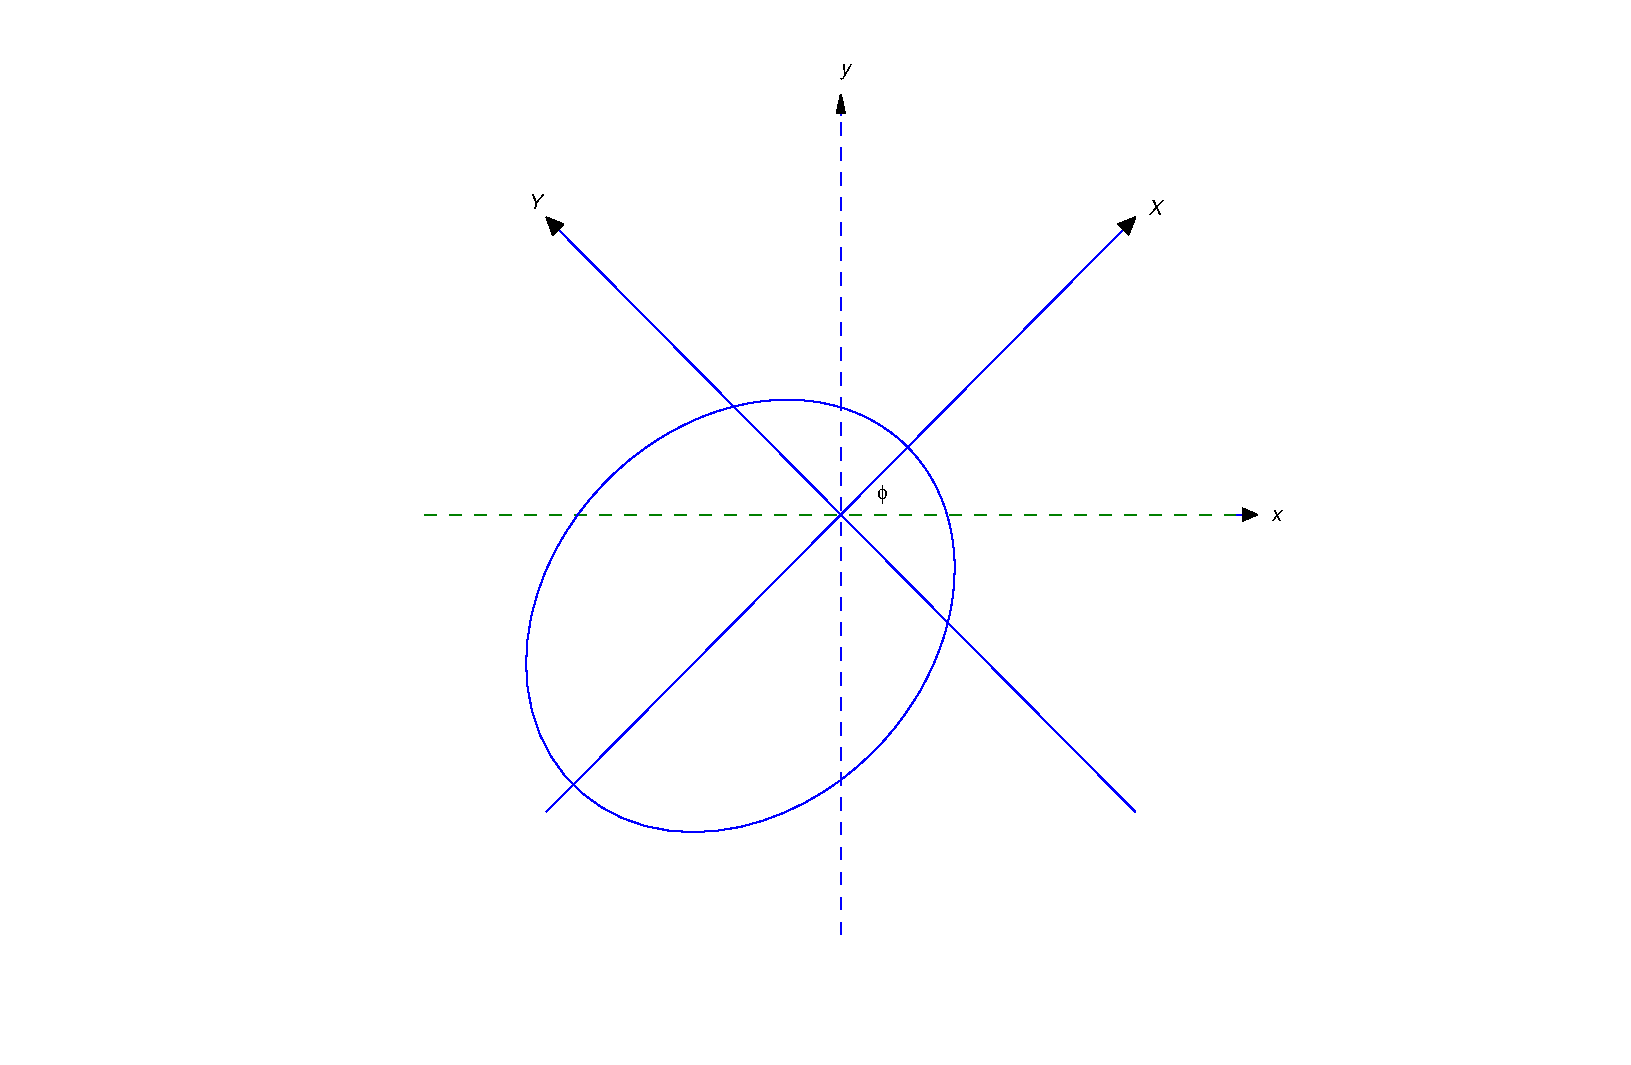
\includegraphics[bb=-78 148 689 643, width=5.67in, height=3.66in, keepaspectratio]{fig060405}
    \color{blue}
    \caption{}
    \label{figure:6.4.5}
  \end{figure}

  \item\label{exer:6.4.2} Suppose an object with mass $m$ moves in the $xy$-plane under the central
        force
  \[
    {\bf F}(r,\theta)=-\frac{mk}{r^{2}}(\cos\theta\,{\bf i}+\sin\theta\,{\bf j}),
  \]
  where $k$ is a positive constant. As we've shown, the orbit of the object is given by
  \[
    r=\frac{\rho}{1+e\cos(\theta-\phi)}.
  \]
  Determine $\rho$, $e$, and $\phi$ in terms of the initial conditions
  \[
    r(0)=r_{0},\quad r'(0)=r_{0}',\text{\; and \;}\theta(0)=\theta_{0},\quad \theta'(0)=\theta_{0}'.
  \]
  Assume that the initial position and velocity vectors are not collinear.

  \item\label{exer:6.4.3} Suppose we wish to put a satellite with mass $m$ into an elliptical orbit
        around Earth. Assume that the only force acting on the object is Earth's gravity, given by
  \[
    {\bf F}(r,\theta)=-mg\left(\frac{R^{2}}{r^{2}}\right)(\cos\theta\,{\bf i}+\sin\theta\,{\bf j}),
  \]
  where $R$ is Earth's radius, $g$ is the acceleration due to gravity at Earth's surface, and $r$
  and $\theta$ are polar coordinates in the plane of the orbit, with the origin at Earth's center.

  \begin{alist}
    \item % (a)
    Find the eccentricity required to make the perigee and apogee distances equal to
    $R\gamma_{1}$ and $R\gamma_{2}$, respectively, where $1<\gamma_{1}<\gamma_{2}$.

    \item % (b)
    Find the initial conditions
    \[
      r(0)=r_{0},\quad r'(0)=r_{0}',\text{\; and \;}\theta(0)=\theta_{0},\quad \theta'(0)=\theta_{0}'
    \]
    required to make the initial point the perigee, and the motion along the orbit in the direction
    of increasing $\theta$. \hint{Use the results of Exercise~\ref{exer:6.4.2}.}
  \end{alist}

  \item\label{exer:6.4.4} An object with mass $m$ moves in a spiral orbit $r=c\theta^{2}$ under a
        central force
  \[
    {\bf F}(r,\theta)=f(r)(\cos\theta\,{\bf i}+\sin\theta\,{\bf j}).
  \]
  Find $f$.

  \item\label{exer:6.4.5} An object with mass $m$ moves in the orbit $r=r_{0}e^{\gamma\theta}$ under
        a central force
  \[
    {\bf F}(r,\theta)=f(r)(\cos\theta\,{\bf i}+\sin\theta\,{\bf j}).
  \]
  Find $f$.

  \item\label{exer:6.4.6} Suppose an object with mass $m$ moves under the central force
  \[
    {\bf F}(r,\theta)=-\frac{mk}{r^{3}}(\cos\theta\,{\bf i}+\sin\theta\,{\bf j}),
  \]
  with
  \[
    r(0)=r_{0},\quad r'(0)=r_{0}',\text{\; and \;}\theta(0)=\theta_{0},\quad \theta'(0)=\theta_{0}',
  \]
  where $h=r_{0}^{2}\theta_{0}'\ne0$.
  \begin{alist}
    \item % (a)
    Set up a second order initial value problem for $u=1/r$ as a function of~$\theta$.

    \item % (b)
    Determine $r=r(\theta)$ if (i) $h^{2}<k$;\; (ii) $h^{2}=k$;\; (iii) $h^{2}>k$.
  \end{alist}
\end{exerciselist}
